\section{System R}

System R ist ein von IBM in den 1970er Jahren durchgeführtes Datenbank Research Projekt \cite{selinger1979access}, \cite{wade2012ibm}, \cite{chamberlin1981history}, \cite{astrahan1976system}, \cite{astrahan1978system}. Es gilt insbesondere auf Grund von zwei Aspekten als der Pinoneer für moderne Datenbanksysteme: Auf der einen Seite wurde in System R zum ersten Mal \ac{SQL} implementiert. Auf der anderen Seite war es das erste System, das die Leistungsfähigkeit von relationalen Datenbanksystemen unter Beweis stellte. Fundamentale Design Entscheidungen, wie dynamische Programmierungsalgorithmen für \ac{QO}, prägen die weitere Entwicklung von Datenbanksystemen. System R gilt als der Vorgänger von IBMs DB2 und als Grundlage für viele andere Datenbanksysteme.


\subsection{Architektur und System Struktur}

\begin{figure}[h]
  \centering
  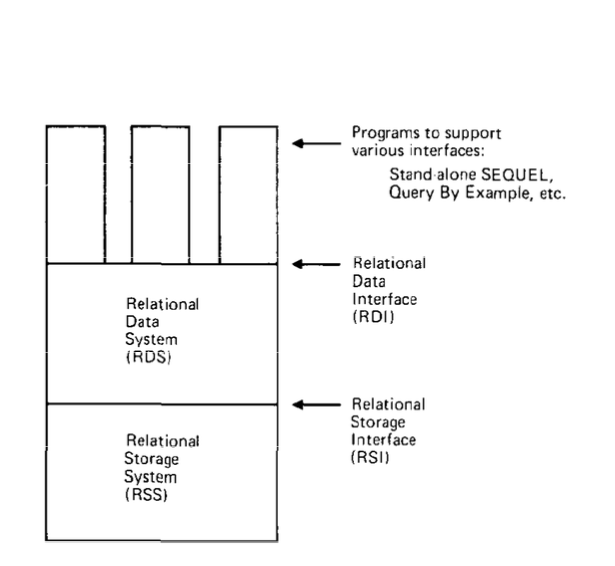
\includegraphics[width=\textwidth]{03_Related_Work/SystemR.png}
  \caption{System R Architektur \cite{astrahan1976system}}
  \label{SystemRArchitecture}
\end{figure}


Wie in Abbildung \ref{SystemRArchitecture} zu erkennen,  besteht das System aus zwei Teilsystemen: \ac{RSS} und \ac{RDS}. 

Das \ac{RSS} ist für die physische Verwaltung der Datenbank verantwortlich. Es kontrolliert u.a. die Speicherverwaltung, das Device-Management, die Transaktionskonsistenz und die Transations- sowie System-Wiederherstellung. Insbesondere fällt in den Aufgabenbereich den Zugriff auf einzelne Tupel von Base Relations. Diese Funktionen werden gegenüber des \ac{RDS} mit Hilfe des \ac{RSI} bereitgestellt.

Das \ac{RDS} übernimmt mit Hife des \ac{RDI} die Kommunikation nach Außen und leitet Befehle über das \ac{RSI} weiter. Anfragen von Außen werden mit Hilfe von \ac{SQL} an das System gestellt. Das \ac{RDS} übernimmt die Umwandlung in ein für das \ac{RSS} verständliche Form und optimiert die Anfrage mit einem Query Optimizer.

Die von IBM verwendeten Begriffe RDS und RSS sind Deckungsgleich mit den Begriffen \ac{CTS} und \ac{RTS}.


\subsection{Verarbeitung von Anfragen}

Wie bei anderen relationalen Datenbanksystemen steht am Beginn eine in \ac{SQL} formulierte Anfrage. Diese Anfrage wird in vier Schritten verarbeitet: Parsen,  Optimieren, Code Generierung und Ausführen.

Im ersten Schritt, Parsen, wird wie bei späteren Systemen die Syntax geprüft und die Anfrage in eine interne Repräsentation umgewandelt. Bei System R werden hierzu Query Blöcke verwendet. Sie repräsentieren die Anfrage mit einer SELECT list, einer FROM list und einem WHERE Baum. Er beinhaltet eine Liste der Elemente, die beispielsweise zum JOIN von Tabellen und der Einschränkung von Datensätzen dienen. Es ist möglich, dass mehrere Query Blöcke für eine einzige Anfrage vorhanden sind. Dies geschieht dann, wenn eine Anfrage Inner-Queries verwendet bzw. Anfragen als Argumente für eine WHERE Bedingung zum Einsatz kommen.


Sobald die Anfrage in Query Blöcke verarbeitet wurde, kommt der \ac{QO} zum Einsatz. Der Optimierer prüft zuerst, ob die genutzten Relationen und Felder auch in der Datenbank vorhanden sind und schlägt Informationen über diese im System R Catalog nach. Teil dieser Informationen sind statistische Informationen der referenzierten Relationen. Diese werden später für die Auswahl der richtigen Access Plans verwendet.

Im nächsten Schritt, optimieren, bestimmt der Optimizer für jeden Query Block den optimalen Access-Pfad. Zuerst wird die Evaluationsreihenfolge der Query Blocks im Statement festgelegt. Dann wird für jeden Query Block die FROM Relationen betrachtet. Sind mehr als eine Relation vorhanden, werden Permutationen der JOIN-Order gebildet. Es wird der Pfad mit den günstigsten Kosten gewählt und die notwendigen Modifikationen werden an der Anfrage vorgenommen. Das Resultat des Prozesses ist ein Plan in der \ac{ASL}.

Nachdem der Plan gefunden und als \ac{ASL}-Tree vorhanden ist, kommt der Code Generator zum Einsatz. Er übersetzt den \ac{ASL}-Plan in einen  Maschinencode. Dieser Code führt die Anfrage des Nutzers auf der Datenbank aus. 

Der Maschinencode wird dann auf dem \ac{RSS} über das \ac{RSI} ausgeführt und das Ergebnis zurückgegeben.

\subsection{Kostenberechnung}
Bei der Auswahl des optimalen Plans beginnt System R mit der Reihenfolge der Query Blocks. Zuerst wird für jeden Query Block geprüft, ob mehrere Tabellen in den FROM Listen vorhanden sind. Falls das der Fall ist, wird die Optimale Join-Order und die Methode des Joins bestimmt. Der Plan mit den geringsten Gesamtkosten für einen Block wird ausgewählt.

Zur Bestimmung der Kosten werden statistische Informationen aus dem System R Catalog herangezogen. Die Berechnung der Kosten für einen Access Plan, werden mit Hilfe der folgenden Funktion abgeschätzt:
$$Cost = Page Fetches + W * (RSI calls)$$


$Page Fetches$ repräsentieren die I/O Operationen, die beispielsweise durch den Abruf der Index Pages und der eigentlichen Pages entsteht. $RSI calls$ ist die Anzahl der erwarteten Datensätze, die durch das \ac{RSS} zurückgegeben werden. Sie dient als Abschätzung wie hoch der CPU Aufwand für die Rückgabe der Werte ist. Mit Hilfe des Parameters $W$ wird eingestellt in welchem Verhältnis I/O zu CPU Kosten stehen.


Bei der Auswahl eines Plans unterscheidet das System zwischen einer „interessanten“ Reihenfolge und einer ungeordneten Reihenfolge. Als interessante Reihenfolge, werden Reihenfolgen betrachtet, die gessanter Reihenfolge“ notwendig sind und die Kosten, die für das lesen in ungeordneter Reihenfolge notwendig sind und addiert auf diese Kosten, die Kosten für das Ordnen der Ergebnisse falls eine ungeordnete Reihenfolge + das Ordnen der Ergebnisse gemeinsam kürzer dauert als das direkte Ausgeben einer interessanten Reihenfolge wird sich für die günstigere Variante entschieden. 

Die Berechnung geschieht auf Daten, die durch den Katalog bereitgestellt werden, Sie enthalten Informationen über die Kardinalität und die Anzahl der Segmente, die für das auslesen einer Relation notwendig sind, ebenfalls wird ein Selektivitätsfaktor genutzt, der das Verhältnis der Gesamtheit zur eingeschlossenen Menge der Anfrage angibt. Spring die Menge der ausgeschlossenen Tupel.



\subsubsection{Plan Transformation}
